%!TEX TS-program = xelatex

\documentclass[t]{beamer}  % [t], [c], или [b] --- вертикальное выравнивание на слайдах (верх, центр, низ)
%\documentclass[t, handout]{beamer} % Раздаточный материал (на слайдах всё сразу)
%\documentclass[aspectratio=169, t]{beamer} % Соотношение сторон

\usepackage{epstopdf}

%\usetheme{Berkeley} % Тема оформления
%\usetheme{Bergen}
%\usetheme{Szeged}

%\usecolortheme{beaver} % Цветовая схема
%\useinnertheme{circles}
%\useinnertheme{rectangles}

\newbool{russian}
\booltrue{russian}  % Загружает русскоязычный логотип ВШЭ
\usepackage{HSE-theme/beamerthemeHSE} % Подгружаем тему



%%% Работа с русским языком
\usepackage{cmap}					% поиск в PDF
\usepackage{mathtext} 				% русские буквы в формулах
\usepackage[T2A]{fontenc}			% кодировка
\usepackage[utf8]{inputenc}			% кодировка исходного текста
%%% Работа с русским языком и шрифтами
\usepackage[english,russian]{babel}   % загружает пакет многоязыковой вёрстки


%%% Дополнительная работа с математикой
\usepackage{amsmath,amsfonts,amssymb,amsthm,mathtools} % AMS
\usepackage{icomma} % "Умная" запятая: $0,2$ --- число, $0, 2$ --- перечисление

%% Номера формул
%\mathtoolsset{showonlyrefs=true} % Показывать номера только у тех формул, на которые есть \eqref{} в тексте.
%\usepackage{leqno} % Нумерация формул слева

%% Свои команды
\DeclareMathOperator{\sgn}{\mathop{sgn}}

%% Перенос знаков в формулах (по Львовскому)
\newcommand*{\hm}[1]{#1\nobreak\discretionary{}
	{\hbox{$\mathsurround=0pt #1$}}{}}

%%% Работа с картинками
\usepackage{graphicx}  % Для вставки рисунков
\graphicspath{{images/}{images2/}}  % папки с картинками
\setlength\fboxsep{3pt} % Отступ рамки \fbox{} от рисунка
\setlength\fboxrule{1pt} % Толщина линий рамки \fbox{}
\usepackage{wrapfig} % Обтекание рисунков текстом
\usepackage{caption}


%%% Работа с таблицами
\usepackage{array,tabularx,tabulary,booktabs} % Дополнительная работа с таблицами
\usepackage{longtable}  % Длинные таблицы
\usepackage{multirow} % Слияние строк в таблице

%%% Программирование
\usepackage{etoolbox} % логические операторы

%%% Другие пакеты
\usepackage{lastpage} % Узнать, сколько всего страниц в документе.
\usepackage{soul} % Модификаторы начертания
\usepackage{csquotes} % Еще инструменты для ссылок
%\usepackage[style=authoryear,maxcitenames=2,backend=biber,sorting=nty]{biblatex}
\usepackage{multicol} % Несколько колонок

%%% Картинки
\usepackage{tikz} % Работа с графикой
\usepackage{pgfplots}
\usepackage{pgfplotstable}
\usepackage{verbatim}
\usetikzlibrary{fadings}
\usepackage[outline]{contour}

\usepackage{chngcntr} % нумерация графиков и таблиц по секциям
\counterwithin{table}{section}
\counterwithin{figure}{section}


\title{Реализация поддержки асинхронного программирования для фреймворка \texttt{DSLab}}
\author{Артём Макогон}
\date{\today}
% \institute[Высшая школа экономики]{National Research University\\ 
	% <<Higher School of Economics>>}

%\input{preamble/preamble}


\begin{document}
	
	\begin{frame}
		\maketitle
	\end{frame}
	

    \section{Введение}
    \subsection{Описание предметной области}


    \begin{frame}
    \frametitle{\insertsection} 
	\framesubtitle{\insertsubsection}

	\begin{figure}
		\centering
		\includegraphics<1>[width=\linewidth]{images/event_pipeline_0}
		\includegraphics<2>[width=\linewidth]{images/event_pipeline_1}
		\includegraphics<3>[width=\linewidth]{images/event_pipeline_2}
		\includegraphics<4>[width=\linewidth]{images/event_pipeline_3}
		\includegraphics<5>[width=\linewidth]{images/event_pipeline_4}
		\includegraphics<6>[width=\linewidth]{images/event_pipeline_5}
		\includegraphics<7>[width=\linewidth]{images/event_pipeline_6}
		\includegraphics<8>[width=\linewidth]{images/event_pipeline_7}
		\includegraphics<9>[width=\linewidth]{images/event_pipeline_8}
		\includegraphics<10>[width=\linewidth]{images/event_pipeline_9}
		\label{simulation}
		\caption*{Исполнение симуляции}
	\end{figure}
        
    \end{frame}

	\subsection{Архитектура проекта DSLab}
	\begin{frame}
		\frametitle{\insertsection} 
		\framesubtitle{\insertsubsection}

		\begin{figure}[H]
			\centering
			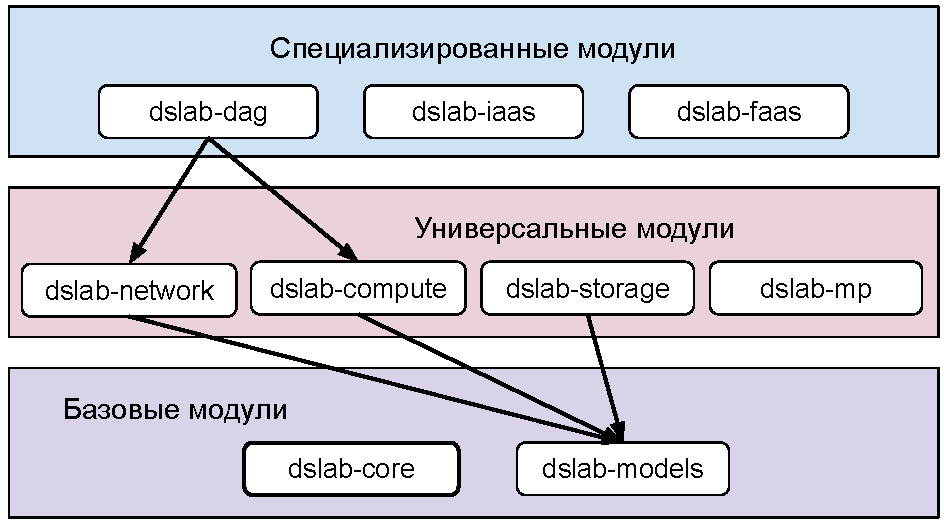
\includegraphics[width=0.9\linewidth]{images/dslab_arc}
			\caption*{Архитектура DSLab}
			\label{dslab_arc}
		\end{figure}
	\end{frame}

	\subsection{\texttt{Callback} модель. Пользовательский код.}
	\begin{frame}
		\frametitle{\insertsection} 
		\framesubtitle{\insertsubsection}

	\end{frame}
\end{document}